\documentclass[10pt,handout]{beamer}

\usepackage{spot}

\usepackage{color}
\definecolor{darkblue}{rgb}{0, 0, .6}
\definecolor{midnightblue}{rgb}{.2, .2, .7}
\definecolor{grey}{rgb}{.7, .7, .7}

\usetheme{Pittsburgh}
\usecolortheme{seahorse}
\useoutertheme{split}

\setbeamertemplate{footline}[split, frame number]
\setbeamertemplate{enumerate items}[default]
\setbeamertemplate{itemize items}[circle]

\newtheorem{comments}{Comments}
\newtheorem{question}{Question}
\newtheorem{goal}{Goal}
\newtheorem{remark}{Remark}
\newtheorem{proposition}{Proposition}
\newtheorem{conjecture}{Conjecture}

\newcommand*\oldmacro{}
\let\oldmacro\insertshorttitle
\renewcommand*\insertshorttitle{
\oldmacro\hfill
\insertframenumber\,/\,\inserttotalframenumber}

%% ----------------------------------------------------------------------  

\begin{document}

\setspotlightstyle{rectangle, rounded corners,fill=structure.fg!25!white,path fading=none}

\title[Inquiry-Based Education in Mathematics]
{\large \textbf{Inquiry-Based Education in Mathematics: Models, Methods, \& Effectiveness for Higher Education}}
\author[D.C.~Ernst and TJ Hitchman]{Dana C.~Ernst, Northern Arizona University\\
Theron Hitchman, University of Northern Iowa}
\institute{\url{http://danaernst.com}\\
\url{http://www.uni.edu/theron/}}

\vspace{1em}

\date{\textbf{Workshop on Innovations in Higher\\ Education Mathematics Teaching}\\
Cardiff University, 7--9 July 2014}

\frame{\titlepage}

%% ----------------------------------------------------------------------

\begin{frame}

\vfill
\begin{center}
\spot[inner sep=3.5ex]{{\Huge \textbf{Why IBL?}}}
\end{center}
\vfill

\end{frame}

%% ----------------------------------------------------------------------

\begin{frame}

\begin{block}{One minute version of why IBL}
\begin{itemize}
\item Our system needs an upgrade.
\item Unintended negative outcomes via traditional methods.
\item Research suggests IBL outcomes are better.
\end{itemize}
\end{block}

\vspace{1em}

\spot{{\large \begin{quote}
``Things my students claim that I taught them masterfully, they don’t know." -- Dylan Retsek
\end{quote}}}

\vspace{1em}

If we really want students to be independent, inquisitive, & persistent, then we need to provide them with the means to acquire these skills.

\end{frame}

%% ----------------------------------------------------------------------

\begin{frame}

\begin{block}{My IBL origins}
\begin{itemize}
\item When I started teaching, I mimicked the experiences I had as a student (i.e., I lectured).
\item By most metrics, I was a successful teacher (e.g., high evaluations, several awards). Why change?
\item Inspired by a Project NExT Workshop run by Carol Schumacher (Kenyon College), I decided to give IBL a try.
\item For 3 consecutive semesters, I taught an intro to proof course at Plymouth State University.
\item 1st two iterations taught via lecture-based approach.
\item 3rd time taught using IBL with emphasis on collaboration.
\item When I taught an abstract algebra course containing students from both styles, anecdotal evidence suggested  students taught via IBL were stronger proof-writers \& more independent as learners.
\item I was sold from that moment on.
\end{itemize}
\end{block}

\end{frame}

%% ----------------------------------------------------------------------

\begin{frame}

\begin{columns}[c]
\column{.7\textwidth}
\begin{block}{Some Data}
\begin{itemize}
\item 2010: 3.7 million students in secondary school. % http://goo.gl/hRixYj
\item 2010: 52\% of those go to University. % http://goo.gl/hwZHYU
\item 2013: 38\% of the UK population had a degree. % http://www.ons.gov.uk/ons/dcp171776_337841.pdf
%\item 2013: 47\% of graduates don't take up graduate jobs. % http://goo.gl/eEQRlh
\item 2010: 16,000 people started a PhD. % http://goo.gl/fcuaqf
\end{itemize}
\end{block}
\column{.2\textwidth}
\begin{center}
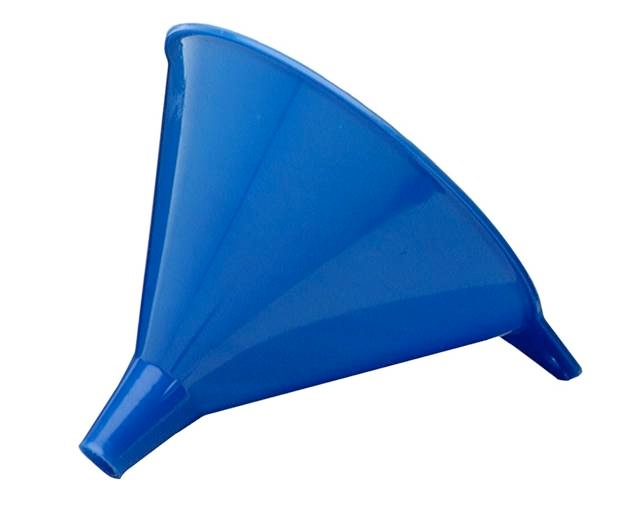
\includegraphics[width=1in]{Funnel.jpg}
\end{center}
\end{columns}

\begin{block}{Conclusion?}
Education is a self-populating institution!
\vspace{1em}
\begin{center}
\spot[inner sep=1.5ex]{{\large \textbf{You are peculiar!}}}
\end{center}
\vspace{1em}
We need to renormalize.

\end{block}

\end{frame}

%% ----------------------------------------------------------------------

\begin{frame}

\begin{block}{What is happening in STEM education?}
\begin{itemize}
\item There exists a growing body of evidence suggesting students are dissatisfied with learning experiences in STEM.
\item Math Education Research suggests that college students have difficulty with:
    \begin{itemize}\normalsize
    \item Solving non-routine problems,
    \item Packing/Unpacking mathematical statements,
    \item Proof.
    \end{itemize}
\end{itemize}

\vspace{1em}

Schoenfeld 1988, Muis 2004, Selden and Selden 1995/1999/2003, Dreyfus 2001, Sowder and Harel 2003, Weber 2001/2003, Weber and Alcock 2004, Tall 1994

\end{block}

\end{frame}

%% ----------------------------------------------------------------------

\begin{frame}

\begin{columns}[c]
\column{.7\textwidth}
\begin{block}{Talking About Leaving}
\begin{itemize}
\item About half of STEM majors switch to non-STEM.
\item Top 4 reasons for switching are teaching related.
\item Good ones leave, too.
\item Loss of interest.
\item Curriculum overload.
\item Students dissatisfied with teaching of STEM classes and less so with non-STEM.
\item Weed-out culture.
\end{itemize}
\end{block}
\column{.2\textwidth}
\begin{center}
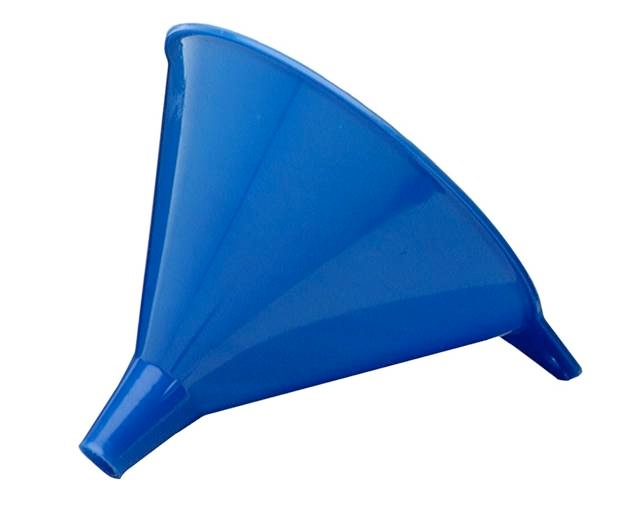
\includegraphics[width=1in]{Funnel.jpg}\\
WRONG PIC
\end{center}
\end{columns}

\end{frame}

%% ----------------------------------------------------------------------

\begin{frame}

\begin{block}{The Good News}
Evidence from the math ed literature suggests that active, learner-centered instruction leads to improved conceptual understanding, problem solving, proof writing, retention, habits of mind, and attitudes about math.

\vspace{1em}

Boaler 1998, Kwon et al. 2005, Rassmussen et al. 2006, Smith 2006, Chappell 2006, Larsen et al. 2011/2013/2014, etc.

\end{block}

\end{frame}

%% ----------------------------------------------------------------------

\begin{frame}

\begin{block}{The Colorado Study}
blah
\end{block}

\end{frame}

%% ----------------------------------------------------------------------

\begin{frame}

\begin{block}{The Twin Pillars}
\begin{enumerate}
\item Deep engagement in rich mathematics,
\item Opportunities to collaborate.
\end{enumerate}

\end{block}

\end{frame}

%% ----------------------------------------------------------------------

\begin{frame}

\begin{block}{Laursen et al. 2013}
\begin{quote}
``Our study indicates that the benefits of active learning experiences may be lasting and significant for some student groups, with no harm done to others. Importantly, ‘covering’ less material in inquiry-based sections had no negative effect on students’ later performance in the major."
\end{quote}

\vspace{1em}

Kogan, M., & Laursen, S. L. (2013).  Assessing long-term effects of inquiry-based learning:  A case study from college mathematics.  Innovative Higher Education, 39(3).
\end{block}

\end{frame}

%% ----------------------------------------------------------------------

\begin{frame}

\begin{block}{Laursen et al. 2014}
\begin{quote}
``blah blah."
\end{quote}

\vspace{1em}

reference???
\end{block}

\end{frame}

%% ----------------------------------------------------------------------

\begin{frame}

\begin{block}{Force Concept Inventory}
blah
\end{block}

\end{frame}

%% ----------------------------------------------------------------------

\end{document}